\chapter{Oxidation and Reduction}\label{ch:g11:redox}

A zinc strip is dipped into a blue solution of copper sulfate. Within
minutes its surface darkens under a spongy, reddish-brown coat; an hour
later the blue of the solution has faded. Copper \omterm{def:g9:periodic-table-first-look:metal}{metal} has appeared
where there was none, and zinc has gone into solution as invisible \omterm{def:g9:ions:ion}{ions}.
Nothing was heated, no gas was given off, no oxygen took part --- and
yet chemists call this an \omterm{def:g11:redox:oxidation}{oxidation}. The word once meant ``combining
with oxygen''; it now means something more general and more useful: the
loss of \omterm{def:g9:inside-the-atom:nucleus}{electrons}. This chapter follows the \omterm{def:g9:inside-the-atom:nucleus}{electrons}.

\begin{recall}
An \omterm{def:g9:ions:ion}{ion} is an \omterm{def:g7:atoms-and-molecules:atom}{atom} or a group of \omterm{def:g7:atoms-and-molecules:atom}{atoms} that has gained or lost \omterm{def:g9:inside-the-atom:nucleus}{electrons}
(\cref{ch:g9:ions}). A \omterm{def:g9:periodic-table-first-look:metal}{metal} such as iron or zinc reacts with
hydrochloric acid to give hydrogen and \omterm{def:g9:periodic-table-first-look:metal}{metal} \omterm{def:g9:ions:ion}{ions}
(\cref{ch:g9:metals-acids-corrosion}). An \omterm{def:g10:the-mole:amount}{amount of substance} $n$, in
\omterm{def:g10:the-mole:amount}{moles}, is computed from a mass $m$ by $n = m/M$
(\cref{ch:g10:the-mole}).
\end{recall}

\begin{omfigure}
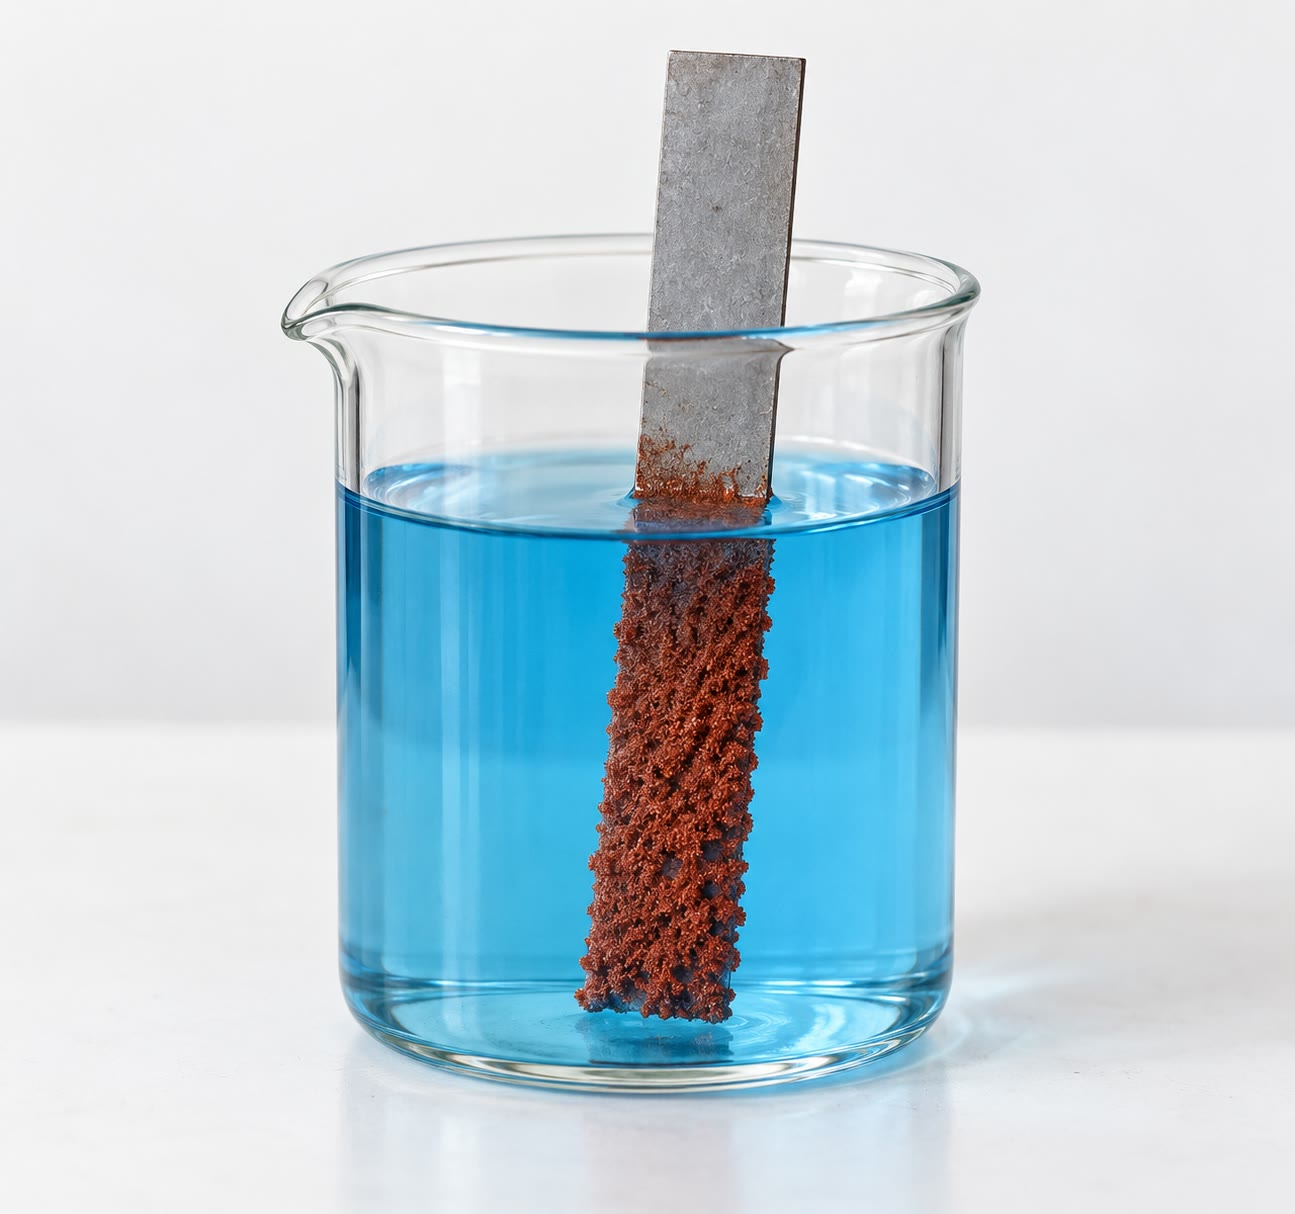
\includegraphics[width=0.55\linewidth]{images/book1/ai/g11-zinc-copper-sulfate.jpg}

{\small A zinc strip in copper sulfate solution: copper is deposited on
the zinc, and zinc \omterm{def:g9:ions:ion}{ions} take its place in the solution.}
\end{omfigure}

\section{Oxidants and reductants}

\begin{definition}[Oxidant and reductant]\label{def:g11:redox:oxidant}
An \emph{oxidant}\index{oxidant} is a species able to gain one or more
\omterm{def:g9:inside-the-atom:nucleus}{electrons}. A \emph{reductant}\index{reductant} is a species able to
give one or more \omterm{def:g9:inside-the-atom:nucleus}{electrons} away.
\end{definition}

\begin{definition}[Oxidation and reduction]\label{def:g11:redox:oxidation}
An \emph{oxidation}\index{oxidation} is a loss of \omterm{def:g9:inside-the-atom:nucleus}{electrons}; a
\emph{reduction}\index{reduction} is a gain of \omterm{def:g9:inside-the-atom:nucleus}{electrons}. A \omterm{def:g11:redox:oxidant}{reductant} is
oxidised; an \omterm{def:g11:redox:oxidant}{oxidant} is reduced.
\end{definition}

\begin{remark}[A way to remember]\label{rem:g11:redox:remember}
In \emph{\omterm{def:g11:redox:oxidation}{reduction}} the charge of the species is reduced: \ce{Cu^{2+}}
gaining two \omterm{def:g9:inside-the-atom:nucleus}{electrons} becomes \ce{Cu}, charge $+2 \to 0$. In an
\omterm{def:g11:redox:oxidation}{oxidation} the charge goes up: \ce{Zn -> Zn^{2+} + 2e-}, $0 \to +2$.
\end{remark}

\begin{definition}[Redox couple and half-equation]\label{def:g11:redox:couple}
An \omterm{def:g11:redox:oxidant}{oxidant} and the \omterm{def:g11:redox:oxidant}{reductant} it becomes by gaining \omterm{def:g9:inside-the-atom:nucleus}{electrons} form a
\emph{redox couple}\index{redox couple}, written Ox/Red with the \omterm{def:g11:redox:oxidant}{oxidant}
first: \ce{Cu^{2+}}/\ce{Cu}, \ce{Zn^{2+}}/\ce{Zn}. The exchange of
\omterm{def:g9:inside-the-atom:nucleus}{electrons} inside a couple is described by its
\emph{half-equation}\index{half-equation},
\[
  \text{Ox} + n\,\ce{e-} \ce{<=>} \text{Red}, % ce-unbalanced-ok (generic form)
\]
balanced in \omterm{def:g7:atoms-and-molecules:atom}{atoms} and in charge, for instance
$\ce{Cu^{2+}(aq) + 2e- <=> Cu(s)}$. The double arrow says that the
exchange can go either way.
\end{definition}

\begin{example}[Metals and their ions]\label{ex:g11:redox:metals}
Every \omterm{def:g9:periodic-table-first-look:metal}{metal} forms a couple with its \omterm{def:g9:ions:ion}{ion}:
\begin{center}
\begin{tabular}{ll}
\hline
couple & \omterm{def:g11:redox:couple}{half-equation} \\
\hline
\ce{Ag+}/\ce{Ag} & \ce{Ag+ + e- <=> Ag} \\
\ce{Cu^{2+}}/\ce{Cu} & \ce{Cu^{2+} + 2e- <=> Cu} \\
\ce{Fe^{2+}}/\ce{Fe} & \ce{Fe^{2+} + 2e- <=> Fe} \\
\ce{Zn^{2+}}/\ce{Zn} & \ce{Zn^{2+} + 2e- <=> Zn} \\
\ce{Al^{3+}}/\ce{Al} & \ce{Al^{3+} + 3e- <=> Al} \\
\hline
\end{tabular}
\end{center}
\omterm{def:g9:ions:ion}{Ions} can form couples too: \ce{Fe^{3+} + e- <=> Fe^{2+}} for the couple
\ce{Fe^{3+}}/\ce{Fe^{2+}}, and \ce{I2 + 2e- <=> 2I-} for
\ce{I2}/\ce{I-}. So can hydrogen: \ce{2H+ + 2e- <=> H2} for
\ce{H+}/\ce{H2}.
\end{example}

\begin{remark}[One species, two roles]\label{rem:g11:redox:amphoteric}
A species can be the \omterm{def:g11:redox:oxidant}{reductant} of one couple and the \omterm{def:g11:redox:oxidant}{oxidant} of another.
The \omterm{def:g9:ions:ion}{ion} \ce{Fe^{2+}} is the \omterm{def:g11:redox:oxidant}{oxidant} of \ce{Fe^{2+}}/\ce{Fe} and the
\omterm{def:g11:redox:oxidant}{reductant} of \ce{Fe^{3+}}/\ce{Fe^{2+}}. Which role it plays depends on
its partner in the reaction.
\end{remark}

\section{Redox reactions}

\begin{definition}[Redox reaction]\label{def:g11:redox:reaction}
A \emph{redox reaction}\index{redox reaction} is a transfer of \omterm{def:g9:inside-the-atom:nucleus}{electrons}
from the \omterm{def:g11:redox:oxidant}{reductant} of one couple to the \omterm{def:g11:redox:oxidant}{oxidant} of another. The
\omterm{def:g11:redox:oxidant}{reductant} is oxidised and the \omterm{def:g11:redox:oxidant}{oxidant} is reduced, at the same time.
\end{definition}

\begin{proposition}[No free electrons]\label{prop:g11:redox:no-free-electrons}
\omterm{def:g9:inside-the-atom:nucleus}{Electrons} do not exist free in a solution: every \omterm{def:g9:inside-the-atom:nucleus}{electron} given by the
\omterm{def:g11:redox:oxidant}{reductant} is taken by the \omterm{def:g11:redox:oxidant}{oxidant}. The equation of a \omterm{def:g11:redox:reaction}{redox reaction} is
therefore obtained by adding the two \omterm{def:g11:redox:couple}{half-equations}, each multiplied by
the number that makes the \omterm{def:g9:inside-the-atom:nucleus}{electrons} given equal to the \omterm{def:g9:inside-the-atom:nucleus}{electrons}
taken; the \omterm{def:g9:inside-the-atom:nucleus}{electrons} then cancel and do not appear in the equation.
\end{proposition}

\begin{example}[Zinc and copper ions]\label{ex:g11:redox:zinc-copper}
In the opening scene the zinc is oxidised and the copper \omterm{def:g9:ions:ion}{ions} are
reduced:
\[
\begin{array}{l@{\qquad}l}
  \ce{Zn(s) -> Zn^{2+}(aq) + 2e-} & \text{(oxidation)}\\
  \ce{Cu^{2+}(aq) + 2e- -> Cu(s)} & \text{(reduction)}\\
  \hline
  \ce{Zn(s) + Cu^{2+}(aq) -> Zn^{2+}(aq) + Cu(s)} &
\end{array}
\]
Two \omterm{def:g9:inside-the-atom:nucleus}{electrons} pass from each zinc \omterm{def:g7:atoms-and-molecules:atom}{atom} to one copper \omterm{def:g9:ions:ion}{ion}. The blue
colour of the solution is the colour of the \ce{Cu^{2+}} \omterm{def:g9:ions:ion}{ions}; it fades
as they are used up, while the colourless \ce{Zn^{2+}} \omterm{def:g9:ions:ion}{ions} take their
place.
\end{example}

\begin{omfigure}
\begin{tikzpicture}[font=\small, >=Stealth,
    ion/.style={circle, draw=black!70, minimum size=10mm, inner sep=0pt}]
  % the zinc strip and the solution
  \fill[black!18] (0,0) rectangle (1.6,4);
  \draw[black!60] (1.6,0) -- (1.6,4);
  \node[anchor=south] at (0.8,0.08) {zinc};
  \fill[omWater!60] (1.6,0) rectangle (9.0,4);
  \node[anchor=north east] at (8.95,3.95) {solution};
  % a zinc atom leaves as an ion
  \node[ion, fill=black!30] (zn) at (1.15,3.0) {\ce{Zn}};
  \node[ion, fill=white] (znion) at (5.0,3.0) {\ce{Zn^{2+}}};
  \draw[->, thick, omProp] (zn.east) -- (znion.west)
    node[midway, above] {oxidation};
  % the electrons travel through the metal
  \draw[->, thick, omDef, dashed] (0.75,2.45) -- (0.75,1.55)
    node[midway, right] {2\,\ce{e-}};
  % a copper ion is reduced on the surface
  \node[ion, fill=omDef!35] (cuion) at (5.0,1.0) {\ce{Cu^{2+}}};
  \node[ion, fill=orange!55!brown] (cu) at (2.12,1.0) {\ce{Cu}};
  \draw[->, thick, omProp] (cuion.west) -- (cu.east)
    node[midway, above] {reduction};
  \node[anchor=west, align=left] at (6.1,2.0) {each zinc atom gives\\ two electrons to one\\ copper ion};
\end{tikzpicture}

{\small At the surface of the zinc. A zinc \omterm{def:g7:atoms-and-molecules:atom}{atom} loses two \omterm{def:g9:inside-the-atom:nucleus}{electrons} and
leaves as a \ce{Zn^{2+}} \omterm{def:g9:ions:ion}{ion}; the two \omterm{def:g9:inside-the-atom:nucleus}{electrons} travel through the \omterm{def:g9:periodic-table-first-look:metal}{metal}
to a \ce{Cu^{2+}} \omterm{def:g9:ions:ion}{ion} touching the surface, which becomes a copper \omterm{def:g7:atoms-and-molecules:atom}{atom}
and stays on the strip.}
\end{omfigure}

\begin{omfigure}
\begin{tikzpicture}[font=\small]
  \pic at (0,0) {beaker={0.75}{omDef!45}};
  \fill[black!35] (-0.15,0.25) rectangle (0.15,2.5);
  \draw[black!65] (-0.15,0.25) rectangle (0.15,2.5);
  \node[anchor=north, align=center] at (0,-0.15) {at the start:\\ blue \ce{Cu^{2+}} solution};
  \draw[->, thick, omProp] (1.3,1) -- (3.2,1) node[midway, above] {one hour};
  \pic at (4.5,0) {beaker={0.75}{omDef!12}};
  \fill[black!35] (4.35,0.25) rectangle (4.65,2.5);
  \fill[orange!55!brown] (4.3,0.25) rectangle (4.7,1.5);
  \draw[black!65] (4.35,0.25) rectangle (4.65,2.5);
  \node[anchor=north, align=center] at (4.5,-0.15) {later: paler solution,\\ copper on the zinc};
\end{tikzpicture}

{\small What can be seen: the deposit of copper on the immersed part of
the strip, and the fading of the blue colour of the \ce{Cu^{2+}} \omterm{def:g9:ions:ion}{ions}.}
\end{omfigure}

\begin{example}[Metals in acid, revisited]\label{ex:g11:redox:acid}
When iron \omterm{def:g2:mixing-and-dissolving:dissolve}{dissolves} in hydrochloric acid, the iron is oxidised and the
\ce{H+} \omterm{def:g9:ions:ion}{ions} are reduced to hydrogen:
\[
  \ce{Fe(s) + 2H+(aq) -> Fe^{2+}(aq) + H2(g)}.
\]
The couples are \ce{Fe^{2+}}/\ce{Fe} and \ce{H+}/\ce{H2}; the chloride
\omterm{def:g9:ions:ion}{ions} take no part.
\end{example}

\begin{inthelab}[The silver tree]
A coil of clean copper wire is hung in a beaker of dilute silver nitrate
solution, \ce{Ag+(aq) + NO3^-(aq)}. Within an hour, branching needles of
shiny silver grow along the wire, and the colourless solution turns
pale blue: \ce{Cu(s) + 2Ag+(aq) -> Cu^{2+}(aq) + 2Ag(s)}. The
experiment is made by the teacher, with gloves and goggles, and the
solution is collected afterwards as hazardous waste.
\end{inthelab}

\begin{safety}{\ghs[0.82cm]{GHS03}\ghs[0.82cm]{GHS05}\ghs[0.82cm]{GHS08}\ghs[0.82cm]{GHS09}}
% ledger: ghs:AgNO3
Silver nitrate: an oxidiser that can feed a fire (GHS03); corrosive to
skin and eyes, and it stains the skin black (GHS05); a health hazard
(GHS08); very toxic to aquatic life, so it never goes down the sink
(GHS09).
\end{safety}

\begin{omfigure}
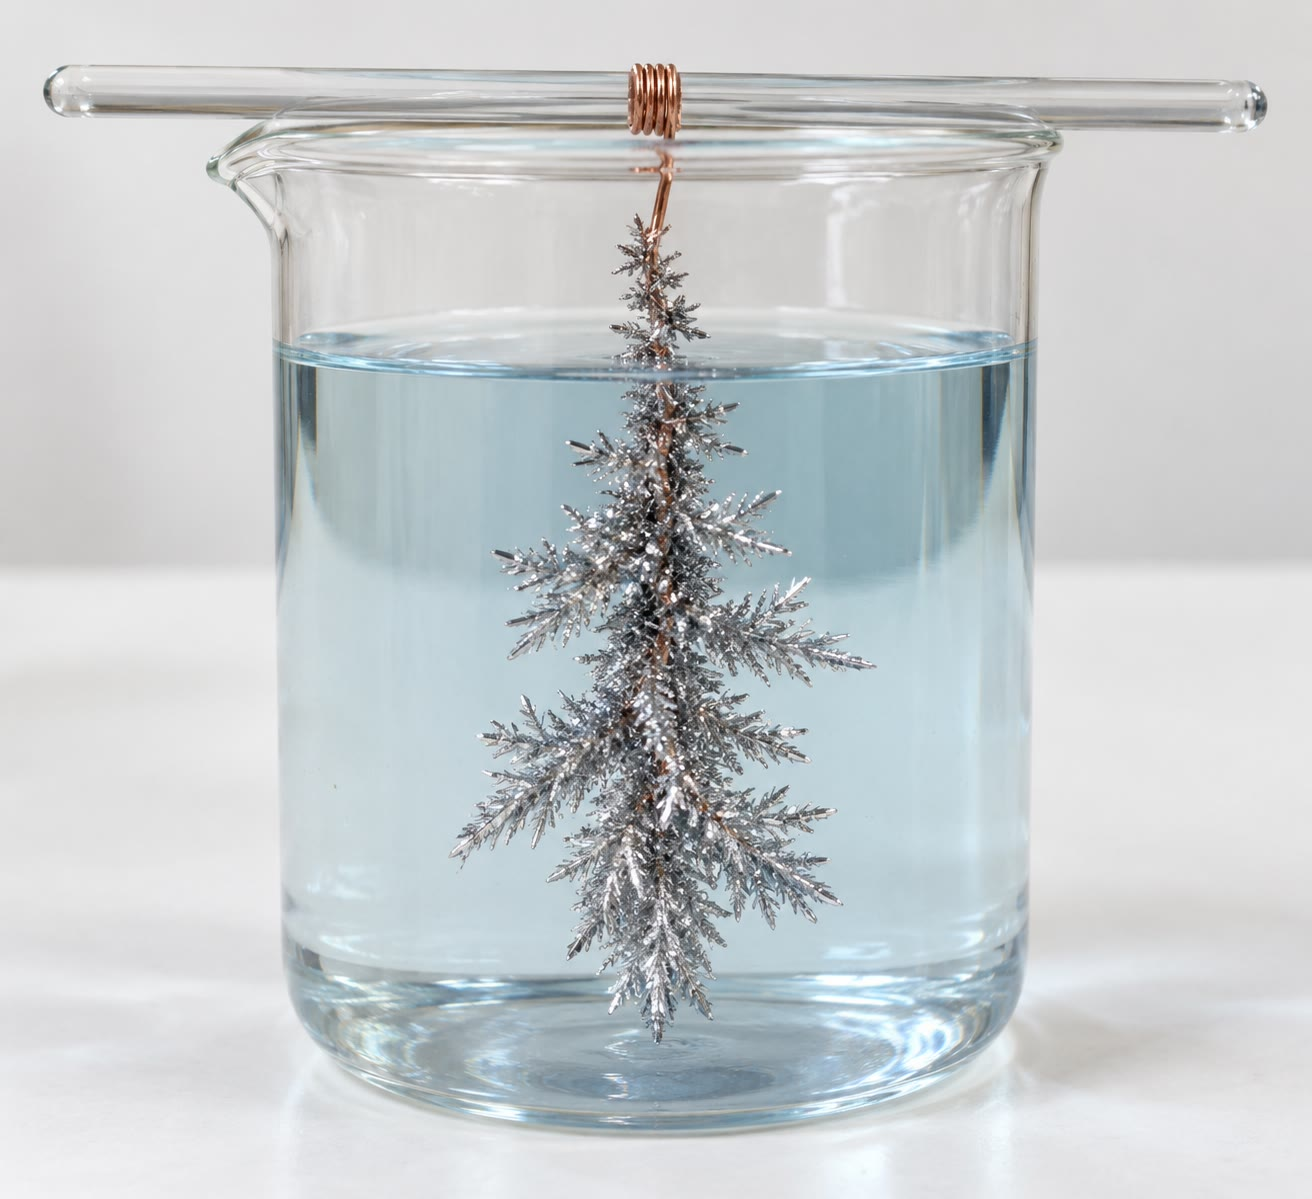
\includegraphics[width=0.5\linewidth]{images/book1/ai/g11-silver-tree.jpg}

{\small Silver crystals growing on a copper wire in silver nitrate
solution.}
\end{omfigure}

\section{Balancing half-equations}

Many important couples contain oxygen and are written for \omterm{def:g9:acids-bases-ph:acidic}{acidic
solutions}, where \ce{H+} \omterm{def:g9:ions:ion}{ions} are present. Their \omterm{def:g11:redox:couple}{half-equations} need
water \omterm{def:g7:atoms-and-molecules:molecule}{molecules} and \ce{H+} \omterm{def:g9:ions:ion}{ions} to balance.

\begin{method}[Balancing a half-equation in acidic solution]\label{met:g11:redox:balance}
To write the \omterm{def:g11:redox:couple}{half-equation} of a couple Ox/Red in \omterm{def:g9:acids-bases-ph:acidic}{acidic solution}:
\begin{enumerate}
  \item write Ox on the left and Red on the right, and balance the \omterm{def:g7:atoms-and-molecules:atom}{atom}
        that is neither O nor H;
  \item balance the oxygen \omterm{def:g7:atoms-and-molecules:atom}{atoms} with water \omterm{def:g7:atoms-and-molecules:molecule}{molecules} \ce{H2O};
  \item balance the hydrogen \omterm{def:g7:atoms-and-molecules:atom}{atoms} with \ce{H+} \omterm{def:g9:ions:ion}{ions};
  \item balance the charge with \omterm{def:g9:inside-the-atom:nucleus}{electrons} \ce{e-}, on the left;
  \item check: same number of each \omterm{def:g7:atoms-and-molecules:atom}{atom}, same total charge on both
        sides.
\end{enumerate}
\end{method}

\begin{example}[The permanganate ion]\label{ex:g11:redox:permanganate}
For the couple \ce{MnO4^-}/\ce{Mn^{2+}} (deep purple to almost
colourless): manganese is balanced; four O on the left give
$\ce{4H2O}$ on the right; their eight H give $\ce{8H+}$ on the left; the
charge on the left is $-1 + 8 = +7$, on the right $+2$, so five
\omterm{def:g9:inside-the-atom:nucleus}{electrons} are added on the left:
\[
  \ce{MnO4^-(aq) + 8H+(aq) + 5e- <=> Mn^{2+}(aq) + 4H2O(l)}.
\]
\end{example}

\begin{example}[The dichromate ion]\label{ex:g11:redox:dichromate}
For \ce{Cr2O7^{2-}}/\ce{Cr^{3+}} (orange to green): two chromium on the
right; seven O give \ce{7H2O}; fourteen H give \ce{14H+}; charge
$-2 + 14 = +12$ on the left against $2 \times 3 = +6$ on the right, so
six \omterm{def:g9:inside-the-atom:nucleus}{electrons}:
\[
  \ce{Cr2O7^{2-}(aq) + 14H+(aq) + 6e- <=> 2Cr^{3+}(aq) + 7H2O(l)}.
\]
\end{example}

\begin{method}[Writing a redox equation]\label{met:g11:redox:combine}
To write the equation of the reaction between the \omterm{def:g11:redox:oxidant}{oxidant} Ox$_1$ of one
couple and the \omterm{def:g11:redox:oxidant}{reductant} Red$_2$ of another:
\begin{enumerate}
  \item write both \omterm{def:g11:redox:couple}{half-equations}, the first in the direction of the
        \omterm{def:g11:redox:oxidation}{reduction} (Ox$_1 \to$ Red$_1$), the second in the direction of
        the \omterm{def:g11:redox:oxidation}{oxidation} (Red$_2 \to$ Ox$_2$);
  \item multiply them by the smallest numbers that make the \omterm{def:g9:inside-the-atom:nucleus}{electrons}
        equal;
  \item add them; the \omterm{def:g9:inside-the-atom:nucleus}{electrons} cancel, and so may some \ce{H+} and
        \ce{H2O} that appear on both sides;
  \item check \omterm{def:g7:atoms-and-molecules:atom}{atoms} and charge once more.
\end{enumerate}
\end{method}

\begin{example}[Permanganate and iron(II)]\label{ex:g11:redox:mno4-fe}
The permanganate \omterm{def:g9:ions:ion}{ion} oxidises \ce{Fe^{2+}} \omterm{def:g9:ions:ion}{ions} to \ce{Fe^{3+}}:
\[
\begin{array}{l@{\qquad}l}
  \ce{MnO4^- + 8H+ + 5e- -> Mn^{2+} + 4H2O} & \times 1\\
  \ce{Fe^{2+} -> Fe^{3+} + e-} & \times 5\\
  \hline
  \ce{MnO4^- + 8H+ + 5Fe^{2+} -> Mn^{2+} + 5Fe^{3+} + 4H2O} &
\end{array}
\]
Charge on the left: $-1 + 8 + 10 = +17$; on the right: $2 + 15 = +17$.
This reaction is used in the next chapter to measure an amount of
iron(II).
\end{example}

\section{Oxidants and reductants around us}

\begin{proposition}[Some common oxidants and reductants]\label{prop:g11:redox:common}
The following species are met again and again in the laboratory and in
everyday life:
\begin{center}
\small
\begin{tabular}{lll}
\hline
species & role & \omterm{def:g11:redox:couple}{half-equation} of its couple \\
\hline
dioxygen \ce{O2} & \omterm{def:g11:redox:oxidant}{oxidant} & \ce{O2 + 4H+ + 4e- <=> 2H2O} \\
dichlorine \ce{Cl2} & \omterm{def:g11:redox:oxidant}{oxidant} & \ce{Cl2 + 2e- <=> 2Cl-} \\
hypochlorite \ce{ClO-} (bleach) & \omterm{def:g11:redox:oxidant}{oxidant} & \ce{2ClO- + 4H+ + 2e- <=> Cl2 + 2H2O} \\
hydrogen peroxide \ce{H2O2} & \omterm{def:g11:redox:oxidant}{oxidant} & \ce{H2O2 + 2H+ + 2e- <=> 2H2O} \\
permanganate \ce{MnO4^-} & \omterm{def:g11:redox:oxidant}{oxidant} & \ce{MnO4^- + 8H+ + 5e- <=> Mn^{2+} + 4H2O} \\
\omterm{def:g9:periodic-table-first-look:metal}{metals} \ce{M} (\ce{Fe}, \ce{Zn}, \ce{Al}\dots) & \omterm{def:g11:redox:oxidant}{reductants} & \ce{M^{n+} + $n$ e- <=> M} % ce-unbalanced-ok (generic)
\\
iodide \ce{I-} & \omterm{def:g11:redox:oxidant}{reductant} & \ce{I2 + 2e- <=> 2I-} \\
thiosulfate \ce{S2O3^{2-}} & \omterm{def:g11:redox:oxidant}{reductant} & \ce{S4O6^{2-} + 2e- <=> 2S2O3^{2-}} \\
ascorbic acid \ce{C6H8O6} (vitamin C) & \omterm{def:g11:redox:oxidant}{reductant} & \ce{C6H6O6 + 2H+ + 2e- <=> C6H8O6} \\
\hline
\end{tabular}
\end{center}
\end{proposition}

\begin{example}[Copper turns green]\label{ex:g11:redox:patina}
Copper roofs and statues, left in the open \omterm{def:g4:air-a-mixture-of-gases:air}{air} for decades, slowly turn
pale green. Oxygen from the \omterm{def:g4:air-a-mixture-of-gases:air}{air} oxidises the copper to \ce{Cu^{2+}} \omterm{def:g9:ions:ion}{ions},
which, with water and carbon dioxide, form a thin green crust, the
patina. Unlike \omterm{def:g9:metals-acids-corrosion:corrosion}{rust} on iron, the patina sticks to the \omterm{def:g9:periodic-table-first-look:metal}{metal} and
protects it from further attack.
\end{example}

\begin{omfigure}

\includegraphics[width=0.48\linewidth]{images/book1/ai/g11-green-roof.jpg}

{\small A copper roof after decades in the \omterm{def:g4:air-a-mixture-of-gases:air}{air}: oxidised copper forms a
green patina.}
\end{omfigure}

\begin{remark}[Antioxidants]\label{rem:g11:redox:antioxidant}
An ``antioxidant'' added to food is a \omterm{def:g11:redox:oxidant}{reductant} that is oxidised by the
oxygen of the \omterm{def:g4:air-a-mixture-of-gases:air}{air} before the food is. Vitamin C (ascorbic acid) is the
commonest: a cut apple sprinkled with lemon juice browns much more
slowly, because the vitamin C of the lemon is oxidised first.
\end{remark}

\section{Exercises}

\begin{exercise}[$\star$]\label{exo:g11:redox:1}
Define an \omterm{def:g11:redox:oxidant}{oxidant}, a \omterm{def:g11:redox:oxidant}{reductant}, an \omterm{def:g11:redox:oxidation}{oxidation} and a \omterm{def:g11:redox:oxidation}{reduction}.
\end{exercise}

\begin{exercise}[$\star$]\label{exo:g11:redox:2}
For each pair, write the \omterm{def:g11:redox:couple}{redox couple} in the form Ox/Red: \ce{Fe} and
\ce{Fe^{2+}}; \ce{Ag} and \ce{Ag+}; \ce{I-} and \ce{I2}; \ce{Fe^{2+}}
and \ce{Fe^{3+}}.
\end{exercise}

\begin{exercise}[$\star$]\label{exo:g11:redox:3}
Write the \omterm{def:g11:redox:couple}{half-equations} of the couples \ce{Ag+}/\ce{Ag},
\ce{Al^{3+}}/\ce{Al}, \ce{Fe^{3+}}/\ce{Fe^{2+}} and \ce{Cl2}/\ce{Cl-}.
\end{exercise}

\begin{exercise}[$\star$]\label{exo:g11:redox:4}
Is the transformation \ce{Fe -> Fe^{2+} + 2e-} an \omterm{def:g11:redox:oxidation}{oxidation} or a
\omterm{def:g11:redox:oxidation}{reduction}? Is iron acting as an \omterm{def:g11:redox:oxidant}{oxidant} or a \omterm{def:g11:redox:oxidant}{reductant}?
\end{exercise}

\begin{exercise}[$\star$]\label{exo:g11:redox:5}
In the reaction \ce{Zn + Cu^{2+} -> Zn^{2+} + Cu}, name the species
oxidised, the species reduced, the \omterm{def:g11:redox:oxidant}{oxidant} and the \omterm{def:g11:redox:oxidant}{reductant}, and give
the number of \omterm{def:g9:inside-the-atom:nucleus}{electrons} transferred for each zinc \omterm{def:g7:atoms-and-molecules:atom}{atom}.
\end{exercise}

\begin{exercise}[$\star\star$]\label{exo:g11:redox:6}
Balance, in \omterm{def:g9:acids-bases-ph:acidic}{acidic solution}, the \omterm{def:g11:redox:couple}{half-equation} of the couple
\ce{H2O2}/\ce{H2O}, following \cref{met:g11:redox:balance} step by
step.
\end{exercise}

\begin{exercise}[$\star\star$]\label{exo:g11:redox:7}
Write the equation of the reaction between iodine \ce{I2} and the
thiosulfate \omterm{def:g9:ions:ion}{ion} \ce{S2O3^{2-}}, which gives iodide \omterm{def:g9:ions:ion}{ions} and
tetrathionate \omterm{def:g9:ions:ion}{ions} \ce{S4O6^{2-}}.
\end{exercise}

\begin{exercise}[$\star\star$]\label{exo:g11:redox:8}
Write the equation of the silver tree reaction from its two
\omterm{def:g11:redox:couple}{half-equations}, and explain why the solution turns blue.
\end{exercise}

\begin{exercise}[$\star\star$]\label{exo:g11:redox:9}
Vitamin C, \ce{C6H8O6}, reacts with iodine \ce{I2}. Write the equation
of the reaction, and say which species is the \omterm{def:g11:redox:oxidant}{reductant}.
\end{exercise}

\begin{exercise}[$\star\star$]\label{exo:g11:redox:10}
Aluminium reacts with copper(II) \omterm{def:g9:ions:ion}{ions}. Write the equation, and explain
why the \omterm{def:g11:redox:couple}{half-equations} must be multiplied by 2 and by 3.
\end{exercise}

\begin{exercise}[$\star\star$]\label{exo:g11:redox:11}
Hydrogen peroxide oxidises iron(II) \omterm{def:g9:ions:ion}{ions} to iron(III) \omterm{def:g9:ions:ion}{ions} in \omterm{def:g9:acids-bases-ph:acidic}{acidic
solution}. Write the equation.
\end{exercise}

\begin{exercise}[$\star\star\star$]\label{exo:g11:redox:12}
A zinc strip loses \qty{1.30}{g} in a solution containing an excess of
copper(II) \omterm{def:g9:ions:ion}{ions}. What mass of copper is deposited? Take
$M(\ce{Zn}) = \qty{65.4}{g/mol}$ and $M(\ce{Cu}) = \qty{63.5}{g/mol}$.
\end{exercise}

\begin{exercise}[$\star\star\star$]\label{exo:g11:redox:13}
Write the equation of the \omterm{def:g11:redox:oxidation}{oxidation} of iron(II) \omterm{def:g9:ions:ion}{ions} by dichromate \omterm{def:g9:ions:ion}{ions}
in \omterm{def:g9:acids-bases-ph:acidic}{acidic solution}. What amount of \ce{Fe^{2+}} is oxidised by
\qty{0.010}{mol} of dichromate \omterm{def:g9:ions:ion}{ions}?
\end{exercise}

\begin{exercise}[$\star\star\star$]\label{exo:g11:redox:14}
Bleach contains hypochlorite \omterm{def:g9:ions:ion}{ions} \ce{ClO-} and chloride \omterm{def:g9:ions:ion}{ions}
\ce{Cl-}. Using the couples \ce{ClO-}/\ce{Cl2} and \ce{Cl2}/\ce{Cl-},
write the equation of the reaction that takes place when bleach meets an
acid, and explain why the labels of bleach and of acidic descaling
products both warn never to \omterm{def:g2:mixing-and-dissolving:mix}{mix} them.
\end{exercise}

\begin{exercise}[$\star\star\star$]\label{exo:g11:redox:15}
In the figure of the zinc surface, the \omterm{def:g9:inside-the-atom:nucleus}{electrons} travel through the
\omterm{def:g9:periodic-table-first-look:metal}{metal}, not through the solution. Using \cref{prop:g11:redox:no-free-electrons},
explain why the copper is deposited on the zinc strip itself and not
elsewhere in the beaker.
\end{exercise}

\section{Problem: The Breath Test}

\begin{problem}[{Weekend problem --- the chemistry of a breath-alcohol
tube: two couples, an orange-to-green colour change, the mass of ethanol
a tube can detect, and the fuel cell that replaced it}]
\label{pb:g11:redox:1}
% ledger: ghs:K2Cr2O7, breath:ratio; molar masses from tools/molar_mass.py
% (0.1-rounded weights): K2Cr2O7 294.2, C2H6O 46.0 g/mol
The first breath-alcohol tests used a glass tube filled with grains of
silica coated with orange potassium dichromate, \ce{K2Cr2O7}, in acid.
Ethanol, \ce{CH3CH2OH}, in the breath blown through the tube reduces the
dichromate \omterm{def:g9:ions:ion}{ions} to green \ce{Cr^{3+}} \omterm{def:g9:ions:ion}{ions} and is oxidised to ethanoic
acid, \ce{CH3COOH}; the length of the green zone measures the ethanol.
Suppose that a tube contains \qty{2.0}{mg} of potassium dichromate. Use
$M(\ce{K}) = 39.1$, $M(\ce{Cr}) = 52.0$, $M(\ce{O}) = 16.0$,
$M(\ce{C}) = 12.0$, $M(\ce{H}) = \qty{1.0}{g/mol}$, $N_A =
\qty{6.02e23}{mol^{-1}}$ and $e = \qty{1.60e-19}{C}$.

\medskip
\noindent\textbf{Part I --- Two couples.}
\begin{enumerate}
  \item Name the two \omterm{def:g11:redox:couple}{redox couples} involved, \omterm{def:g11:redox:oxidant}{oxidant} first.
  \item Is ethanol oxidised or reduced? Is it the \omterm{def:g11:redox:oxidant}{oxidant} or the
        \omterm{def:g11:redox:oxidant}{reductant}?
  \item Write the \omterm{def:g11:redox:couple}{half-equation} of the couple
        \ce{Cr2O7^{2-}}/\ce{Cr^{3+}} in \omterm{def:g9:acids-bases-ph:acidic}{acidic solution}.
  \item Write the \omterm{def:g11:redox:couple}{half-equation} of the couple
        \ce{CH3COOH}/\ce{CH3CH2OH} in \omterm{def:g9:acids-bases-ph:acidic}{acidic solution}.
  \item Deduce the equation of the reaction in the tube.
\end{enumerate}

\medskip
\noindent\textbf{Part II --- What one tube can measure.}
\begin{enumerate}[resume]
  \item Explain the colour change of the grains.
  \item Compute the \omterm{def:g10:the-mole:molar-mass}{molar mass} of potassium dichromate.
  \item Compute the amount of dichromate \omterm{def:g9:ions:ion}{ions} in the tube.
  \item What amount of ethanol is needed to turn the whole tube green?
  \item Deduce the largest mass of ethanol one tube can measure.
\end{enumerate}

\medskip
\noindent\textbf{Part III --- From breath to blood.}
A person blows \qty{1.0}{L} of breath through the tube; the green zone
grows in proportion to the mass of ethanol that reaches it.
\begin{enumerate}[resume]
  \item The breath contains \qty{0.25}{mg} of ethanol per litre. What
        fraction of the dichromate is used?
  \item The tube is \qty{10}{cm} long. How long is the green zone?
  \item Breath analysers assume that \qty{2100}{L} of breath carry as
        much ethanol as \qty{1}{L} of blood. Estimate the mass of ethanol
        per litre of blood, in grams.
  \item Why does the green zone start at the inlet of the tube and grow
        towards the outlet, instead of the whole tube turning slightly
        green?
  \item Why can a tube be used only once?
\end{enumerate}

\medskip
\noindent\textbf{Part IV --- The \omterm{def:g4:what-a-fire-needs:fuel}{fuel} cell.}
Potassium dichromate carries the pictograms
\ghs[0.6cm]{GHS03}\,\ghs[0.6cm]{GHS05}\,\ghs[0.6cm]{GHS06}\,\ghs[0.6cm]{GHS07}\,\ghs[0.6cm]{GHS08}\,\ghs[0.6cm]{GHS09}.
Modern devices use instead a \omterm{def:g4:what-a-fire-needs:fuel}{fuel} cell, in which the ethanol of the
breath is oxidised by dioxygen on an electrode, and the \omterm{def:g9:inside-the-atom:nucleus}{electrons}
released flow through a wire.
\begin{enumerate}[resume]
  \item Give two reasons, read from the pictograms, why dichromate
        tubes were abandoned.
  \item Write the equation of the \omterm{def:g11:redox:oxidation}{oxidation} of ethanol by dioxygen,
        using the couple \ce{O2}/\ce{H2O}.
  \item How many \omterm{def:g9:inside-the-atom:nucleus}{electrons} does one ethanol \omterm{def:g7:atoms-and-molecules:molecule}{molecule} give up when it is
        oxidised to ethanoic acid?
  \item For \qty{0.25}{mg} of ethanol, compute the amount of ethanol,
        then the number of \omterm{def:g9:inside-the-atom:nucleus}{electrons} released.
  \item Deduce the electric charge that flows through the \omterm{def:g4:what-a-fire-needs:fuel}{fuel} cell.
        Why is this charge a good measure of the ethanol in the breath?
\end{enumerate}
\end{problem}
